\documentclass[a4paper]{article}

  \usepackage{fullpage} % Package to use full page
  \usepackage{parskip} % Package to tweak paragraph skipping
  \usepackage{tikz} % Package for drawing
  \usepackage{amsmath}
  \usepackage{siunitx} % Package for scientific units
  \usepackage{amsfonts}
  \usepackage{amssymb}
  \usepackage{hyperref}
  \usepackage[utf8]{inputenc}
  \usepackage[english]{babel}
  \usepackage{multicol}
  \usepackage{graphicx} % Package for including images
  \graphicspath{ {./images/} }
  
  \newcommand\tab[1][0.5cm]{\hspace*{#1}}
  
  \title{Assignment 2}
  \author{Adrian Darian}
  \date{9/4/2020}
  
  \begin{document}
  
\maketitle
  
\section*{Chapter 2}
\begin{itemize}
	\item[6] Consider the interconnection shown in the figure below. \\
	      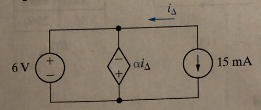
\includegraphics{P2-6.png} \\ 
	      \begin{itemize}
	      	\item[a)] What value of $\alpha$ is required to make this a valid interconnection?
	      	\item[b)] For this value of $\alpha$, find the power associated with the current source.
	      	\item[c)] Is the current source supplying or absorbing power?
	      \end{itemize} 
	\item[9] Find the total power developed in the circuit in the figure below if $v_{o} = \SI{5}{\volt}$ \\
	      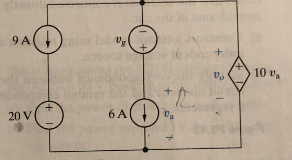
\includegraphics{P2-9.png} \\
	\item[15] A variety of current source values were applied to the device shown in the figure below \\
	      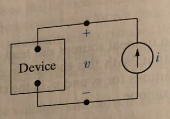
\includegraphics{P2-15.png} \\
	      \begin{tabular}{|c|c|}
	      	\hline
	      	$i\si{\milli\ampere}$ & $p\si{\milli\watt}$ \\
	      	\hline
	      	$0.5$                 & $8.25$              \\
	      	\hline
	      	$1.0$                 & $33.00$             \\
	      	\hline
	      	$1.5$                 & $74.25$             \\
	      	\hline
	      	$2.0$                 & $132.00$            \\
	      	\hline
	      	$2.5$                 & $206.25$            \\
	      	\hline
	      	$3.0$                 & $297.00$            \\
	      	\hline
	      \end{tabular}
	\item[18] Given the circuit shown in the figure below, find \\
	      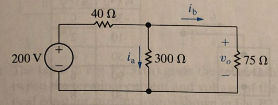
\includegraphics{P2-18.png} \\	  
	      \begin{itemize}
	      	\item[a)] the value of $i_{a}$
	      	\item[b)] the value of $i_{b}$
	      	\item[c)] the value of $v_{o}$
	      	\item[d)] the power dissipated in each resistor
	      	\item[e)] the power delivered by the $\SI{200}{\volt}$ source    
	      \end{itemize}
	\item[24] The currents $i_{1}$ and $i_{2}$ in the circuit in the figure below are $\SI{20}{\ampere}$ and $\SI{15}{\ampere}$, respectively \\
	      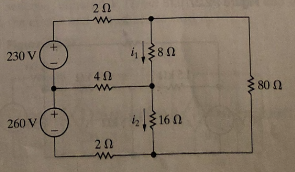
\includegraphics{P2-24.png} \\	  
	      \begin{itemize}
	      	\item[a)] Find the power supplied by each voltage source.
	      	\item[b)] Show that the total power supplied equals the total power dissipated in the resistors. 
	      \end{itemize}
	\item[32] Consider the circuit shown in the figure below. \\
	      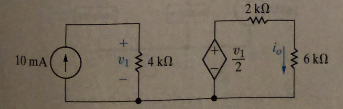
\includegraphics{P2-32.png} \\	  
	      \begin{itemize}
	      	\item[a)] Find $i_{o}$
	      	\item[b)] Verify the value of $i_{o}$ by showing that the power generated in the circuit equals the power absorbed in the circuit. 
	      \end{itemize}  
\end{itemize}

  
\end{document}